\PassOptionsToPackage{hypertexnames=false}{hyperref}
\documentclass[a4paper,fleqn]{cas-sc}
\renewcommand{\sfdefault}{\rmdefault}
\input{glyphtounicode}
\pdfgentounicode=1

\usepackage[numbers,sort&compress]{natbib}
\usepackage{booktabs}
\usepackage{float}
\usepackage{multirow}
\usepackage{amsmath,amssymb}
\usepackage{xcolor}

\begin{document}
\let\WriteBookmarks\relax
\let\printorcid\relax
\def\floatpagepagefraction{1}
\def\textpagefraction{.001}
\shorttitle{Supplementary Material}
\shortauthors{M.S. Hasan et al.}

\title[mode=title]{Supplementary Material for When do dark-water pseudo-labels help test-time adaptation in SAR flood mapping?}
\author[1]{MD Sakib Hasan}
\author[1]{Mostofa Seum}
\author[1]{Meer Mursalin}
\author[1]{Tanvir Ahmed}
\cormark[1]
\ead{tanvir.ahmed@aiub.edu}
\author[1]{Rifath Mahmud}
\author[1]{Syeda Anika Tasnim}
\affiliation[1]{organization={Department of Computer Science, American International University-Bangladesh (AIUB)},
            city={Dhaka}, country={Bangladesh}}
\cortext[1]{Corresponding author}
\begin{abstract}
The supplement covers calibration, historical benchmarks and external score verification.
\end{abstract}
\maketitle

\renewcommand{\thesection}{S\arabic{section}}
\renewcommand{\thefigure}{S\arabic{figure}}
\renewcommand{\thetable}{S\arabic{table}}
\renewcommand{\theequation}{S\arabic{equation}}

\section{Flood-level miss-rate calibration}
\label{sec:calib}
These historical experiments use conformal risk control for mean miss rate and split conformal calibration for the share of events meeting a miss target. Related flood applications include optical prediction sets and density-aware SAR risk control \citep{konidakis2025cpflood,li2026crcflood}. The external comparisons in the main article use fixed source thresholds.
For each method we store, per event, the histogram of predicted water probabilities (1000 bins) separately for water and dry pixels. This gives, for every threshold $t_k=k/1000$, the event's miss rate $\mathrm{FNR}_e(t_k)$. Each flood contributes one loss curve for calibration. This choice allows spatial dependence among pixels within an event. The theoretical statements require exchangeability across the event loss curves. We use two rules, both computed from $n$ labelled calibration floods.

\paragraph{Mean rule.} Following conformal risk control \citep{angelopoulos2024crc}, the threshold is
\begin{equation}
\hat{k}_{\mathrm{mean}} = \max\Big\{k : \frac{n}{n+1}\,\frac{1}{n}\sum_{i=1}^{n}\mathrm{FNR}_i(t_k) + \frac{1}{n+1} \le \alpha\Big\}.
\label{eq:mean}
\end{equation}
Because FNR is bounded by 1 and does not increase as the threshold falls, $\mathbb{E}[\mathrm{FNR}_{n+1}(t_{\hat{k}})]\le\alpha$ when the calibration floods and the new flood are exchangeable. This bounds the miss rate averaged over floods. It says nothing about a single flood, and individual floods can miss far more than $\alpha$.

\paragraph{Per-flood rule.} To make a statement about each flood, let $k_i=\max\{k:\mathrm{FNR}_i(t_k)\le\alpha\}$ be the highest threshold at which calibration flood $i$ still meets the target. The threshold is the $\lfloor\delta(n+1)\rfloor$-th smallest of $k_1,\dots,k_n$ (and $0$, mapping everything as water, if $\lfloor\delta(n+1)\rfloor=0$). By the standard split-conformal argument \citep{vovk2022alrw,lei2018distfree}, a new exchangeable flood then meets the target with probability at least $1-\delta$:
\begin{equation}
\mathbb{P}\big[\mathrm{FNR}_{n+1}(t_{\hat{k}_{\mathrm{flood}}})\le\alpha\big]\ \ge\ 1-\delta .
\label{eq:flood}
\end{equation}
We report $\alpha=0.2$ with $\delta=0.2$ (at least four floods in five miss at most 20\% of their water) and $\delta=0.1$. The price is a lower threshold and therefore more false alarms than under the mean rule.

\paragraph{Scope of the theoretical statements.} The statements above require exchangeable loss curves under a fixed prediction/adaptation procedure. The Sen1Floods11 curves here are generated by different leave-one-event-out fitted models, while external events use the source-trained models. We report this cross-fitted transfer empirically; we have not established that the standard split-conformal proof covers this exact fitted-model protocol. The per-flood probability is marginal over calibration and a new event, not a conditional guarantee for every particular flood or a high-confidence guarantee for a realised calibration set.

\paragraph{Where the calibration floods come from.} Both statements hold only if the calibration floods are exchangeable with the new one. We evaluate two settings. In \emph{same-dataset} calibration each event is calibrated on all other events of its dataset (leave one flood out); this uses labels of other floods from the target dataset and is the favourable case. In \emph{source-only} calibration the thresholds are computed once, on the 11 Sen1Floods11 floods, and applied unchanged to another dataset, so that no label of the target dataset is used at any point. Exchangeability is then not assured \citep{tibshirani2019covshift,barber2023beyond}, and whether the target is met becomes an empirical question that depends on how comparable the model's scores are across datasets.

\section{Historical results and calibration diagnostics}\label{sec:historical}

\paragraph{Historical comparator implementations.} TENT-R retains running batch-normalisation statistics for final inference. Reference TENT forces batch statistics. EATA-inspired omits redundancy filtering and estimates its Fisher penalty on target batches. SAR-inspired omits the recovery mechanism. CoTTA-inspired always averages four SAR-augmented teacher predictions and omits the source-confidence gate. These names refer to custom implementations throughout the historical results. The controlled normalisation comparison appears in Appendix A of the main article.
Within each controlled comparison, the adaptation methods start from the same models and use the same crops, batch size and number of steps (200).
\begin{itemize}
\item \textbf{No adaptation}, and \textbf{AdaBN} alone \citep{li2018adabn}.
\item \textbf{Entropy minimisation on batch-norm weights}: TENT-R \citep{wang2021tent} (Adam, learning rate $10^{-3}$); EATA-inspired \citep{niu2022eata}, which uses only reliable pixels (entropy below $0.4\ln 2$), re-weights them and anchors the weights with a Fisher penalty (estimated here with the unadapted model on the first 20 target batches); and SAR-inspired \citep{niu2023sar}, which adds sharpness-aware updates ($\rho=0.05$) to the reliable-pixel loss.
\item \textbf{Teacher--student self-training}: plain self-training with an exponential-moving-average teacher, following \citet{chen2026cimttda}; and CoTTA-inspired \citep{wang2022cotta}, which averages the teacher over augmentations (flips and backscatter offsets), trains all weights on the soft teacher output and restores 1\% of the weights to their source values at every step.
\item \textbf{Physics-checked self-training}, without AdaBN and after AdaBN, with either fixed thresholds ($-18$\,dB VV, $-25$\,dB VH, relative height and slope) or the adaptive rule of the main article's Methods. AdaBN followed by the adaptive rule is the proposed method.
\item \textbf{Model-free references}: an Otsu threshold on VV \citep{otsu1979threshold}, and on Kuro Siwo a change-detection rule that uses the pre-flood image: a pixel is flood water if it is dark after the flood (below the per-flood dark threshold) and its VV dropped by more than the Otsu threshold of the difference image, capped at $-3$\,dB \citep{giustarini2013change,clement2018multitemporal}.
\item \textbf{Supervised reference}: same-dataset calibration uses labelled floods of the target dataset, so we also ask what those labels buy when used for training. The Kuro Siwo events were split into five folds by event; each source model was fine-tuned on the labelled chips of four folds (1,500 steps, Adam, learning rate $10^{-4}$) and tested on the events of the fifth. The recipe was fixed in advance and not tuned.
\end{itemize}
Historical TENT-R and AdaBN were run on Sen1Floods11, Kuro Siwo and MMFlood. EATA-inspired, SAR-inspired, CoTTA-inspired and the supervised reference were run on Kuro Siwo only; the historical plain self-training arm was run on Sen1Floods11 and Kuro Siwo. Kuro Siwo distinguishes permanent water from flood water. The main scores count both as water, as Sen1Floods11 does; a second set of scores ignores permanent-water pixels (``flood water only'').

\paragraph{Follow-up implementation audits.} Separately verified \texttt{baselines\_v2} runs used corrected TENT, EATA and SAR implementations and are archived outside the historical tables. The controlled tiled-inference audit is reported in Appendix A of the main paper. A later Kuro Siwo radar and terrain validity-mask correction did not establish a reliable improvement and is omitted from the main results.

\subsection{Sen1Floods11, leave one flood out}
On held-out Sen1Floods11 floods, the in-domain setting, all methods except TENT-R lie within 0.03 IoU of each other (Table~\ref{tab:s1f}), and no difference between the proposed method and no adaptation or AdaBN is significant with 11 floods. TENT-R is the weakest at every threshold. With only 10 calibration floods the mean rule is conservative: at the 20\% target the realised mean miss rate is 0.12--0.13, and IoU drops by about 0.07 relative to threshold 0.5. Targets below $1/(n+1)\approx0.09$ cannot be met with an informative threshold, because the correction term alone exceeds them (Fig.~\ref{fig:guarantee}a, d).

\begin{table}[pos=t]
\caption{Sen1Floods11, leave one flood out (11 floods, radar only): mean IoU at threshold 0.5, under the mean rule (Eq.~\ref{eq:mean}) and under the per-flood rule (Eq.~\ref{eq:flood}), with the number of floods that meet the 20\% target under the per-flood rule. Best value per column in bold.}
\label{tab:s1f}
\centering
\small
\begin{tabular}{lcccccc}
\toprule
 & & \multicolumn{3}{c}{Mean rule, target $\alpha$} & \multicolumn{2}{c}{Per-flood rule, $\alpha=\delta=0.2$} \\
\cmidrule(lr){3-5}\cmidrule(lr){6-7}
Method & 0.5 & 10\% & 20\% & 30\% & IoU & Floods meeting \\
\midrule
No adaptation & 0.551 & 0.189 & 0.479 & 0.543 & \textbf{0.475} & 9.0/11 \\
Self-training \citep{chen2026cimttda} & 0.550 & 0.193 & 0.486 & 0.551 & 0.461 & 9.0/11 \\
TENT-R (running statistics) & 0.504 & 0.168 & 0.442 & 0.527 & 0.405 & 9.0/11 \\
AdaBN & 0.573 & 0.182 & 0.479 & 0.562 & 0.459 & 9.0/11 \\
Physics-checked self-training, fixed rule & 0.566 & 0.193 & 0.491 & 0.565 & 0.465 & 9.0/11 \\
Physics-checked self-training, adaptive rule & 0.556 & 0.150 & \textbf{0.497} & 0.551 & 0.463 & 9.0/11 \\
AdaBN + physics check, fixed rule & \textbf{0.575} & \textbf{0.195} & 0.481 & \textbf{0.571} & 0.439 & 9.0/11 \\
AdaBN + physics check, adaptive rule (proposed) & 0.561 & 0.171 & 0.494 & 0.557 & 0.459 & 9.0/11 \\
\bottomrule
\end{tabular}

\end{table}

\subsection{Kuro Siwo}
The domain gap is large (Table~\ref{tab:ks}): without adaptation the models miss 81\% of the water at threshold 0.5 (IoU 0.186). Same-dataset calibration alone recovers much of the gap (0.565 at the 20\% target), because the threshold moves to where the new dataset needs it; this gain comes from labels of other Kuro Siwo floods and not from adaptation. The fair comparison between adaptation methods is therefore at a calibrated threshold, where their mean miss rates are approximately equal (0.17 at the 20\% target, Fig.~\ref{fig:guarantee}e). There, none of the six historical variants has an established significant gain over the unadapted model. AdaBN, EATA-inspired, SAR-inspired and CoTTA-inspired are level with it (0.558--0.574 against 0.565; no difference is significant), and plain self-training and TENT-R are worse (0.457 and 0.467). At threshold 0.5, by contrast, TENT-R, EATA-inspired, SAR-inspired, CoTTA-inspired and AdaBN all look strong (0.563--0.598 against 0.186): what they gain at 0.5 is the operating point that calibration provides anyway. The physics-guided arm reached 0.677 IoU at the nominal target in this historical comparison. The internal entropy and restoration variants used simplified implementations. The observed difference widened at stricter nominal targets (0.565 at the 10\% target against 0.456 without adaptation and 0.327--0.436 for the baselines). These custom variants differ from the reference TTA algorithms. Inference normalisation and realised miss rates can affect these comparisons.

\paragraph{Supervised reference.} Fine-tuning the source models on the labelled chips of other Kuro Siwo events reaches 0.661 IoU at threshold 0.5 and 0.657 at the 20\% target. The proposed method, which uses no Kuro Siwo label for adaptation, has an observed IoU of 0.677 versus 0.657; equivalence was not tested ( better on 11 of 26 events, $p=0.71$), and its observed miss rates are more even: under the mean rule its worst event misses 38\% of the water, against 64\% for the fine-tuned models. Fine-tuning is ahead at the strictest target (0.592 against 0.565 at 10\%). The fine-tuning recipe was not tuned, so this is a reference point and not an upper bound on what target labels can give.

\begin{table}[pos=t]
\caption{Kuro Siwo, 26 unseen events, U-Net trained on Sen1Floods11, radar only, same-dataset calibration (mean over three models): mean IoU at threshold 0.5, under the mean rule and under the per-flood rule, with the number of floods that meet the 20\% target under the per-flood rule. Bold marks leading neural network IoUs among the label-free methods. A fractional number of floods meeting the target is the average of the three model-level counts. The Otsu row uses its own VV threshold. The fine-tuned models use labels of other Kuro Siwo events.}
\label{tab:ks}
\centering
\small
\begin{tabular}{lcccccc}
\toprule
 & & \multicolumn{3}{c}{Mean rule, target $\alpha$} & \multicolumn{2}{c}{Per-flood rule, $\alpha=\delta=0.2$} \\
\cmidrule(lr){3-5}\cmidrule(lr){6-7}
Method & 0.5 & 10\% & 20\% & 30\% & IoU & Floods meeting \\
\midrule
No adaptation & 0.186 & 0.456 & 0.565 & 0.550 & 0.529 & 21.7/26 \\
Self-training \citep{chen2026cimttda} & 0.174 & 0.360 & 0.457 & 0.490 & 0.432 & 21.3/26 \\
TENT-R (running statistics) & 0.576 & 0.327 & 0.467 & 0.576 & 0.413 & 21.3/26 \\
EATA-inspired & 0.563 & 0.410 & 0.558 & 0.565 & 0.530 & 21.3/26 \\
SAR-inspired & 0.598 & 0.374 & 0.564 & 0.590 & 0.517 & 21.0/26 \\
CoTTA-inspired & 0.583 & 0.436 & 0.574 & 0.587 & 0.554 & 21.0/26 \\
AdaBN & 0.570 & 0.399 & 0.562 & 0.584 & 0.535 & 21.0/26 \\
Physics-checked self-training, adaptive rule & 0.627 & 0.500 & 0.666 & \textbf{0.655} & 0.577 & 21.0/26 \\
AdaBN + physics check, fixed rule & 0.669 & 0.525 & 0.664 & 0.649 & 0.624 & 21.0/26 \\
AdaBN + physics check, adaptive rule (proposed) & \textbf{0.673} & \textbf{0.565} & \textbf{0.677} & 0.644 & \textbf{0.652} & 21.0/26 \\
\midrule
Fine-tuned on labelled target floods (supervised) & 0.661 & 0.592 & 0.657 & 0.638 & 0.643 & 21.3/26 \\
\midrule
Otsu threshold on VV (no model) & 0.456 & -- & -- & -- & -- & -- \\
\bottomrule
\end{tabular}

\end{table}

\paragraph{What each part contributes.} Physics-checked self-training without AdaBN reaches almost the same IoU as the full method under the mean rule (0.666 against 0.677; $p=0.71$). AdaBN matters elsewhere: at threshold 0.5 (0.627 against 0.673), for the worst flood (the method without AdaBN misses up to 85\% of the water on one event, the full method at most 38\%; Table~\ref{tab:transfer}), under the per-flood rule (0.577 against 0.652; better on 24 of 26 events, $p=6\times10^{-6}$) and, most of all, when no target labels are available for calibration (Section~\ref{sec:transfer}). The two parts therefore do different jobs: the physics check recovers water the model misses, and re-estimating the batch-norm statistics makes the scores comparable from flood to flood and from dataset to dataset, which is what a shared threshold needs.

Fig.~\ref{fig:guarantee} shows the whole trade-off for the mean rule. The plotted mean miss rates are empirical observations. A shared nominal target can yield different realised miss rates, especially at strict settings where the procedure maps all pixels as water.

\begin{figure}[pos=t]
\centering
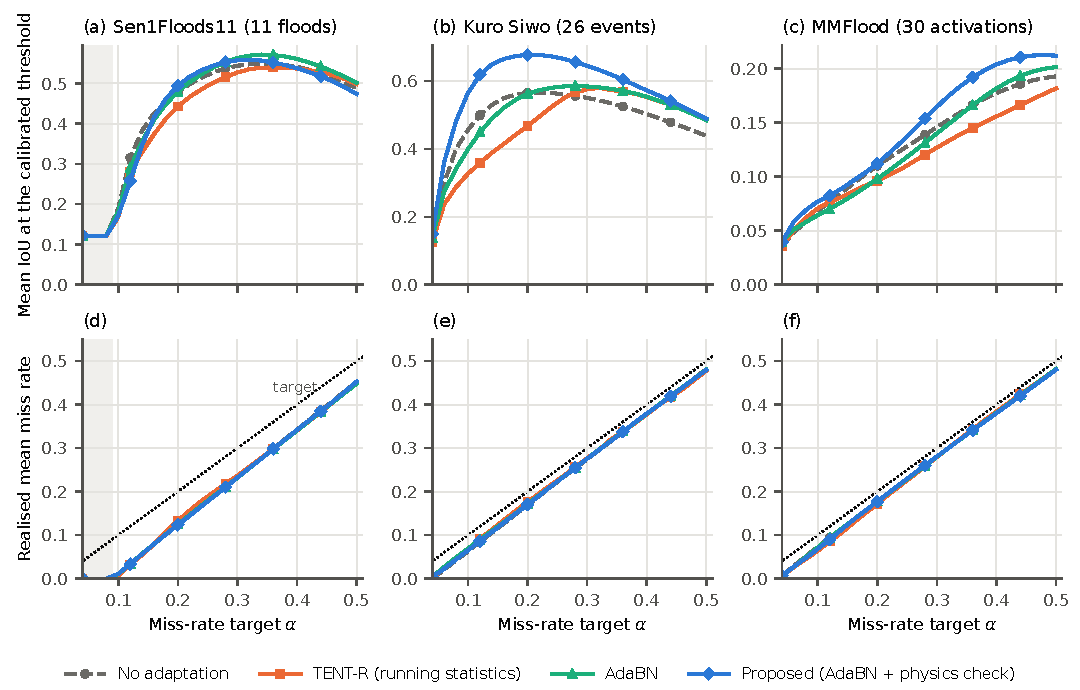
\includegraphics[width=\textwidth]{figures/fig_guarantee.pdf}
\caption{Observed accuracy and miss rate under the mean rule with same-dataset calibration as the miss-rate target $\alpha$ varies. (a--c) Mean IoU at the calibrated threshold; (d--f) realised mean miss rate, with the target as a dotted line. Sen1Floods11: 11 floods, leave one flood out; Kuro Siwo: 26 events; MMFlood: 30 activations; mean over three models for the last two. Shading: targets below $1/(n+1)$ cannot be met with an informative threshold.}
\label{fig:guarantee}
\end{figure}

Per event (Fig.~\ref{fig:ksevents}), the mean hides a wide spread: at the 20\% target, between 16 and 20 of the 26 events meet the target under the mean rule, depending on the method. The baselines occasionally fail badly: on their worst event AdaBN, EATA-inspired and SAR miss 85--88\% of the water, TENT-R 92\% and CoTTA-inspired 74\%. The worst event of the proposed method misses 38\%.

\begin{figure}[pos=t]
\centering
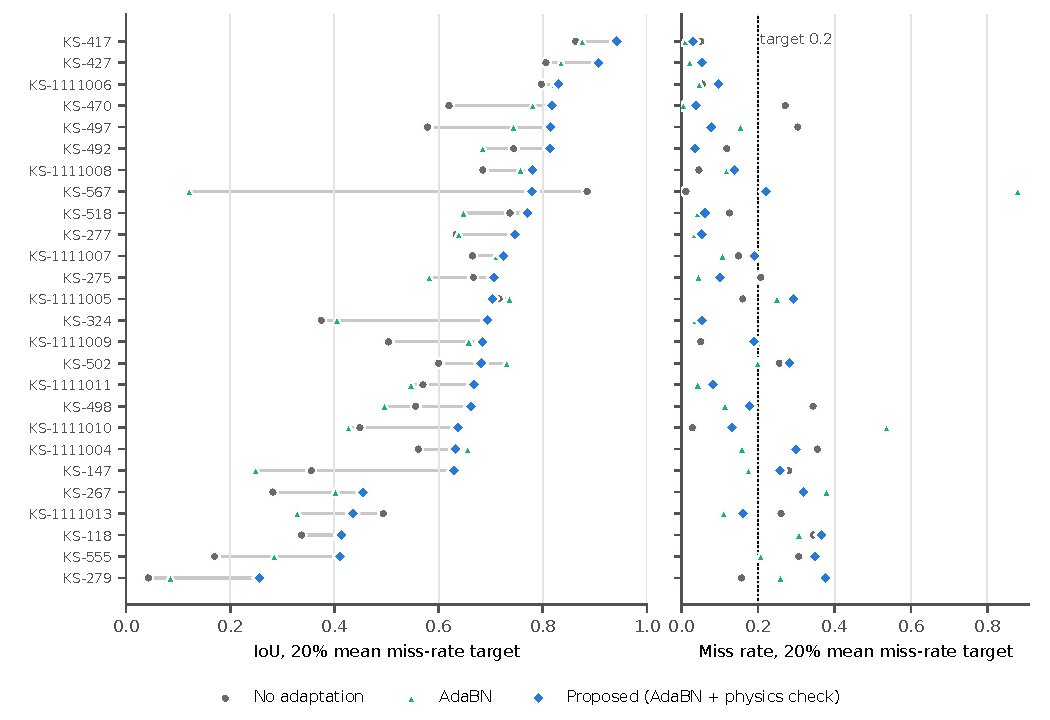
\includegraphics[width=\textwidth]{figures/fig_ks_events.pdf}
\caption{Kuro Siwo, per event, mean rule at the 20\% target with same-dataset calibration (mean over three models): IoU (left) and miss rate (right) without adaptation, with AdaBN, and with the proposed method. Events are sorted by the IoU of the proposed method.}
\label{fig:ksevents}
\end{figure}

The physics check also produces cleaner maps (Table~\ref{tab:prec}). At a common miss-rate target the proposed method has the highest precision (0.780, against 0.504--0.768 for the other rows) and the lowest false-alarm rate (2.5\% of dry pixels, against 3.8--8.9\%). At threshold 0.5 the unadapted model is precise but misses 81\% of the water.

\begin{table}[pos=t]
\caption{Kuro Siwo (26 events, three U-Net models): mean miss rate, precision and false-alarm rate (share of dry pixels mapped as water) at threshold 0.5 and under the mean rule at the 20\% target.}
\label{tab:prec}
\centering
\small
\begin{tabular}{lcccccc}
\toprule
 & \multicolumn{3}{c}{Threshold 0.5} & \multicolumn{3}{c}{Mean rule, 20\% target} \\
\cmidrule(lr){2-4}\cmidrule(lr){5-7}
Method & Miss rate & Precision & False alarms & Miss rate & Precision & False alarms \\
\midrule
No adaptation & 0.806 & 0.844 & 0.3\% & 0.169 & 0.644 & 6.8\% \\
Self-training & 0.818 & 0.867 & 0.3\% & 0.167 & 0.504 & 8.9\% \\
TENT-R (running statistics) & 0.335 & 0.854 & 1.6\% & 0.176 & 0.555 & 7.0\% \\
EATA-inspired & 0.178 & 0.668 & 4.3\% & 0.172 & 0.659 & 4.5\% \\
SAR-inspired & 0.240 & 0.755 & 2.5\% & 0.173 & 0.664 & 4.2\% \\
CoTTA-inspired & 0.179 & 0.690 & 3.5\% & 0.172 & 0.677 & 3.8\% \\
AdaBN & 0.177 & 0.674 & 3.9\% & 0.171 & 0.663 & 4.1\% \\
Physics check only & 0.322 & 0.904 & 1.2\% & 0.171 & 0.768 & 3.5\% \\
Proposed & 0.152 & 0.760 & 2.9\% & 0.170 & 0.780 & 2.5\% \\
\bottomrule
\end{tabular}

\end{table}

\paragraph{Flood water only.} The scores above count permanent water as water, and permanent water is the easy part of the task. Table~\ref{tab:ksf} repeats the comparison with permanent-water pixels ignored. Every method loses about 0.10 IoU and the order does not change: at the 20\% target the proposed method reaches 0.565, against 0.460 without adaptation and 0.350--0.471 for TENT-R, EATA-inspired, SAR-inspired, CoTTA-inspired and AdaBN and it is level with the fine-tuned models (0.581; $p=0.26$ before correction). One advantage does not carry over. With permanent water ignored, the worst event of the proposed method misses 75\% of its flood water under the mean rule, within the range of the baselines (66--89\%), so the even miss rates seen above partly reflect permanent water that every flood contains.

\begin{table}[pos=t]
\caption{Kuro Siwo scored on flood water only (permanent-water pixels ignored), 26 events, three U-Net models, same-dataset calibration; columns as in Table~\ref{tab:ks}. Historical runs on floodwater-only support. Bold marks leading label-free neural network IoUs. Flood counts are averaged across seeds.}
\label{tab:ksf}
\centering
\small
\begin{tabular}{lcccccc}
\toprule
 & & \multicolumn{3}{c}{Mean rule, target $\alpha$} & \multicolumn{2}{c}{Per-flood rule, $\alpha=\delta=0.2$} \\
\cmidrule(lr){3-5}\cmidrule(lr){6-7}
Method & 0.5 & 10\% & 20\% & 30\% & IoU & Floods meeting \\
\midrule
No adaptation & 0.158 & 0.365 & 0.460 & 0.466 & 0.444 & 21.0/26 \\
TENT-R (running statistics) & 0.481 & 0.265 & 0.350 & 0.441 & 0.327 & 21.7/26 \\
EATA-inspired & 0.473 & 0.357 & 0.469 & 0.484 & 0.438 & 21.0/26 \\
SAR-inspired & 0.502 & 0.317 & 0.455 & 0.496 & 0.429 & 21.3/26 \\
CoTTA-inspired & 0.485 & 0.369 & 0.471 & 0.495 & 0.439 & 21.0/26 \\
AdaBN & 0.473 & 0.337 & 0.461 & 0.495 & 0.416 & 21.0/26 \\
AdaBN + physics check, adaptive rule (proposed) & \textbf{0.569} & \textbf{0.439} & \textbf{0.565} & \textbf{0.570} & \textbf{0.534} & 21.0/26 \\
\midrule
Fine-tuned on labelled target floods (supervised) & 0.597 & 0.503 & 0.581 & 0.590 & 0.549 & 21.0/26 \\
\bottomrule
\end{tabular}

\end{table}

\paragraph{Model-free references and the pre-flood image.} A single Otsu threshold on VV reaches 0.456 IoU. The darkness test of the physics check used alone, a per-event dark threshold on VV with no model, reaches 0.560 on all water and 0.532 on flood water only, at a miss rate of 34\%. Adding the pre-flood image (dark after the flood and a drop in VV larger than the change threshold) removes permanent water as intended but also loses flood water: 0.527 IoU on flood water at a miss rate of 42\%, and 0.399 on all water. At threshold 0.5 the proposed method is above these references (0.673 on all water, 0.569 on flood water) at about half their miss rate (15\% and 18\%). On flood water the margin over the plain dark threshold is small in IoU (0.04), which shows how much of the Kuro Siwo task the darkness cue alone carries; these references have no score to calibrate, so the comparison is not at a common miss-rate target.

Fig.~\ref{fig:maps} shows maps for four Kuro Siwo events, each on the chip with the most labelled water, at the threshold of the mean rule for the 20\% target. On event 324 the unadapted model and the proposed method map the flooded field cleanly, whereas TENT-R and AdaBN add false alarms along its edge. On event 1111010, a chip almost entirely under water, TENT-R misses 90\% of the water while the other methods miss almost none. On event 147 all methods agree. Event 118 shows the typical failure: every method misses water in narrow channels and at field margins, and here TENT-R misses the least (12\% against 26\% for the proposed method).

\begin{figure}[pos=t]
\centering
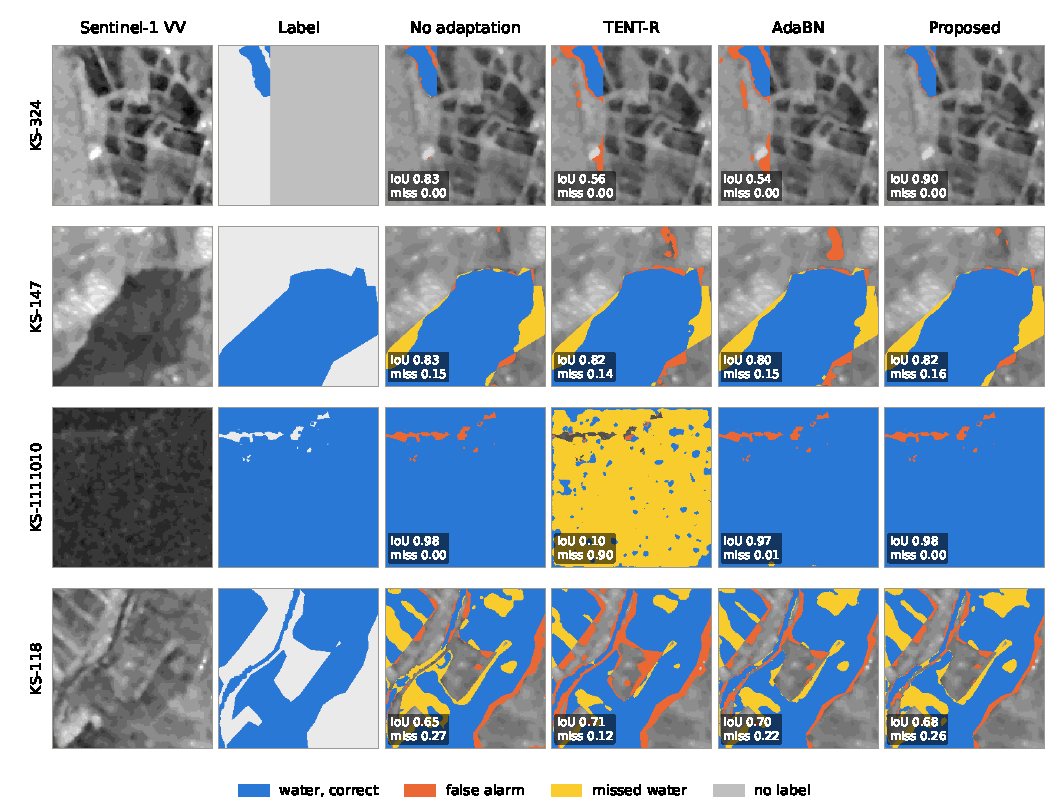
\includegraphics[width=\textwidth]{figures/fig_maps_audited.pdf}
\caption{Example maps on Kuro Siwo (U-Net model seed 0, radar only) at the mean-rule threshold for the 20\% target, calibrated on the other events. Columns: Sentinel-1 VV (2$\times$2 averaged and quantised for display), label, and the maps of each method coloured by agreement with the label; IoU and miss rate refer to the shown chip. Grey label areas are unlabelled and not scored.}
\label{fig:maps}
\end{figure}

\subsection{Calibration without target labels}
\label{sec:transfer}
Same-dataset calibration needs labelled floods from the target dataset, which an emergency mapper may not have. Table~\ref{tab:transfer} and Fig.~\ref{fig:transfer} therefore repeat the comparison with thresholds calibrated once, on the 11 Sen1Floods11 floods, and applied unchanged. No Kuro Siwo or MMFlood label is used.

On Kuro Siwo the result depends entirely on adaptation. Without adaptation the source-calibrated threshold fails: the models miss 58\% of the water on average against a target of 20\%, and an average of 2.7 of 26 events per seed meet the target. After any adaptation that re-estimates or trains the batch-norm layers, the target is met with a wide margin (mean miss rate 0.06--0.07). The proposed method is more accurate than the other two (IoU 0.557, against 0.426 for AdaBN and 0.346 for TENT-R; $+0.132$ over AdaBN, better on 25 of 26 events, Holm-corrected $p=10^{-6}$; $+0.211$ over TENT-R, 26 of 26, $p=3\times10^{-7}$) and the most even across floods: an average of 25.0 of 26 events per seed meet the target and the worst misses 23\% of its water, against 58--59\% for AdaBN and TENT-R. Because the realised miss rate is well below the target, the 30\% target is the more efficient operating point: there the proposed method reaches 0.672 IoU at a mean miss rate of 0.148 with a mean count of 24 of 26 events meeting the 30\% target, which is the accuracy it reaches with same-dataset calibration. Physics-checked self-training without AdaBN reaches a higher IoU at the 20\% target (0.662), because its realised mean miss rate (0.156) sits closer to the target, but it is not reliable in this setting: an average of 19.7 of 26 events per seed meet the target, one event misses 78\% of its water, and at the 30\% target the mean miss rate exceeds the target (0.321). The picture is the same with permanent water ignored: the source-calibrated threshold misses 62\% of the flood water without adaptation and 7\% with the proposed method (IoU 0.446 against 0.336 for AdaBN and 0.268 for TENT-R). EATA-inspired, SAR-inspired and CoTTA-inspired were not run on Sen1Floods11, so we omit source-calibrated thresholds for those historical variants.

On MMFlood source-only calibration does not hold. At the 20\% target the realised mean miss rate is 0.28 without adaptation, 0.24 with AdaBN and 0.26 with the proposed method; only TENT-R stays below the target (0.19), at the lowest IoU. Calibrating on Sen1Floods11 and Kuro Siwo together (37 floods) does not help the adapted models either (mean miss rate 0.34--0.38). This result offers little support for treating Sen1Floods11 floods and MMFlood activations as exchangeable after adaptation. Section~\ref{sec:historical_errors} examines potential contributors. Whether a source-calibrated threshold can be trusted on a new dataset therefore has to be checked, not assumed; on MMFlood the miss-rate statements of this paper hold only with same-dataset calibration.

\begin{table}[pos=t]
\caption{Where the calibration floods come from: mean rule at the 20\% target, calibrated on the other floods of the same dataset or on the 11 Sen1Floods11 floods only (no label of the target dataset). Mean IoU, mean miss rate, worst seed-averaged flood miss rate, and number of floods meeting the target. Counts are averaged across three seeds. Mean miss rates above the target are in italics.}
\label{tab:transfer}
\centering
\small
\setlength{\tabcolsep}{4pt}
\resizebox{\textwidth}{!}{\begin{tabular}{llcccccccc}
\toprule
 & & \multicolumn{4}{c}{Same-dataset calibration} & \multicolumn{4}{c}{Source-only calibration (Sen1Floods11)} \\
\cmidrule(lr){3-6}\cmidrule(lr){7-10}
Dataset & Method & IoU & Miss & Worst & Meeting & IoU & Miss & Worst & Meeting \\
\midrule
Kuro Siwo & No adaptation & 0.565 & 0.169 & 0.35 & 15.7/26 & 0.366 & \textit{0.583} & 0.95 & 2.7/26 \\
 & TENT-R (running statistics) & 0.467 & 0.176 & 0.92 & 19.7/26 & 0.346 & 0.073 & 0.59 & 23.3/26 \\
 & AdaBN & 0.562 & 0.171 & 0.88 & 17.7/26 & 0.426 & 0.072 & 0.58 & 23.7/26 \\
 & Physics check only & 0.666 & 0.171 & 0.85 & 19.0/26 & 0.662 & 0.156 & 0.78 & 19.7/26 \\
 & Proposed & 0.677 & 0.170 & 0.38 & 17.0/26 & 0.557 & 0.062 & 0.23 & 25.0/26 \\
\midrule
MMFlood & No adaptation & 0.110 & 0.176 & 0.72 & 21.0/30 & 0.150 & \textit{0.280} & 0.82 & 16.3/30 \\
 & TENT-R (running statistics) & 0.096 & 0.172 & 0.57 & 19.7/30 & 0.103 & 0.186 & 0.61 & 18.7/30 \\
 & AdaBN & 0.098 & 0.177 & 0.65 & 20.0/30 & 0.128 & \textit{0.242} & 0.74 & 17.3/30 \\
 & Proposed & 0.112 & 0.177 & 0.77 & 19.7/30 & 0.157 & \textit{0.256} & 0.90 & 17.0/30 \\
\bottomrule
\end{tabular}
}
\end{table}

\begin{figure}[pos=t]
\centering
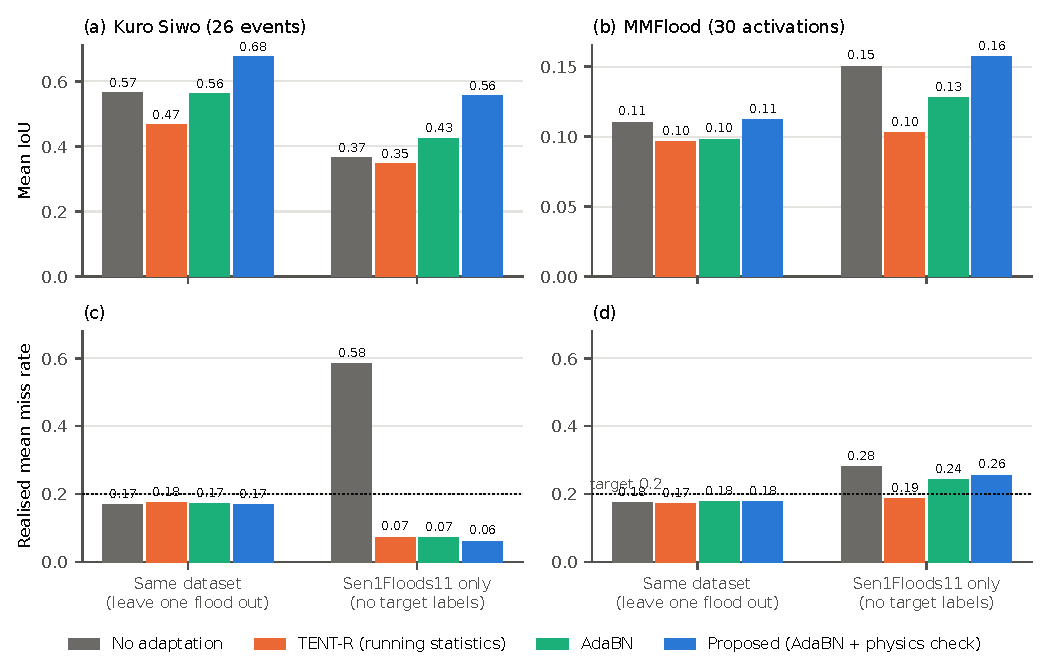
\includegraphics[width=\textwidth]{figures/fig_transfer.pdf}
\caption{Mean IoU (a, b) and realised mean miss rate (c, d) under the mean rule at the 20\% target, with same-dataset calibration and with calibration on Sen1Floods11 only. On Kuro Siwo the source-calibrated threshold fails without adaptation and holds after it; on MMFlood it fails for three of the four methods.}
\label{fig:transfer}
\end{figure}

\subsection{Per-flood rule}
\label{sec:perflood}
The mean rule leaves a third of the floods above the target. The per-flood rule (Eq.~\ref{eq:flood}) trades accuracy for coverage (Table~\ref{tab:perflood}). With same-dataset calibration and $\delta=0.2$, between 80\% and 83\% of the floods miss at most 20\% of their water on the three calibration benchmarks for every method evaluated there, for the entries in the table. With $\delta=0.1$ the observed share is 90--92\%. On Kuro Siwo the proposed method keeps an IoU of 0.652 under this stricter rule, close to its 0.677 under the mean rule, whereas no adaptation, AdaBN and TENT-R fall to 0.529, 0.535 and 0.413, and EATA-inspired, SAR-inspired and CoTTA-inspired to 0.517--0.554. It remains level with the fine-tuned models (0.643). On MMFlood all methods are within 0.011 IoU of each other. The nominal $\delta$ concerns a new exchangeable event. Individual floods above the target can still have high miss rates.

\begin{table}[pos=t]
\caption{Per-flood rule at $\alpha=0.2$ with same-dataset calibration: mean IoU, number (share) of floods that miss at most 20\% of their water, and the worst event miss rate after seed averaging. Counts are averaged across three seeds for Kuro Siwo and MMFlood.}
\label{tab:perflood}
\centering
\small
\resizebox{\textwidth}{!}{\begin{tabular}{llcccccc}
\toprule
 & & \multicolumn{3}{c}{$\delta=0.2$ (at least 80\% of floods)} & \multicolumn{3}{c}{$\delta=0.1$ (at least 90\% of floods)} \\
\cmidrule(lr){3-5}\cmidrule(lr){6-8}
Dataset & Method & IoU & Meeting & Worst & IoU & Meeting & Worst \\
\midrule
Sen1Floods11 & No adaptation & \textbf{0.475} & 9.0/11 (82\%) & 0.26 & \textbf{0.447} & 10.0/11 (91\%) & 0.24 \\
 & TENT-R (running statistics) & 0.405 & 9.0/11 (82\%) & 0.48 & 0.345 & 10.0/11 (91\%) & 0.25 \\
 & AdaBN & 0.459 & 9.0/11 (82\%) & 0.27 & 0.402 & 10.0/11 (91\%) & 0.26 \\
 & Proposed & 0.459 & 9.0/11 (82\%) & 0.34 & 0.360 & 10.0/11 (91\%) & 0.26 \\
\midrule
Kuro Siwo & No adaptation & 0.529 & 21.7/26 (83\%) & 0.23 & 0.500 & 24.0/26 (92\%) & 0.21 \\
 & TENT-R (running statistics) & 0.413 & 21.3/26 (82\%) & 0.84 & 0.287 & 24.0/26 (92\%) & 0.45 \\
 & AdaBN & 0.535 & 21.0/26 (81\%) & 0.83 & 0.315 & 24.0/26 (92\%) & 0.61 \\
 & Proposed & \textbf{0.652} & 21.0/26 (81\%) & 0.28 & \textbf{0.615} & 24.0/26 (92\%) & 0.26 \\
\midrule
MMFlood & No adaptation & 0.082 & 24.0/30 (80\%) & 0.65 & 0.061 & 27.0/30 (90\%) & 0.48 \\
 & TENT-R (running statistics) & 0.077 & 24.3/30 (81\%) & 0.39 & 0.068 & 27.3/30 (91\%) & 0.36 \\
 & AdaBN & 0.072 & 25.0/30 (83\%) & 0.39 & 0.063 & 27.3/30 (91\%) & 0.27 \\
 & Proposed & \textbf{0.083} & 24.7/30 (82\%) & 0.36 & \textbf{0.074} & 27.0/30 (90\%) & 0.29 \\
\bottomrule
\end{tabular}
}
\end{table}

\subsection{MMFlood: internally planned final test}
\label{sec:mm}
The protocol was written locally before the MMFlood download. After download and before seeing results, we fixed the activation as the statistical unit. At a nominal 20\% mean miss target with same-dataset calibration, H1 and H2 compare physics-guided adaptation against TENT-R and AdaBN. H3 compares it against no adaptation at threshold 0.5. H4 asks whether the observed mean miss rate is at most 0.20. H1--H3 use one-sided signed-rank tests with Holm correction. Overlapping leave-one-activation-out calibration sets induce dependence.
Table~\ref{tab:mm} reports the primary analysis on 30 activations with same-dataset calibration. Of the four internally planned hypotheses, three are supported and one is not. H1 and H2 are supported: under the mean rule at the 20\% target the proposed method beats TENT-R by 0.016 IoU (better on 28 of 30 activations, Holm-adjusted $p=5.59\times10^{-8}$) and AdaBN by 0.014 (28 of 30, Holm-adjusted $p=5.59\times10^{-8}$). H3 is not supported: at threshold 0.5 the mean gain over no adaptation is 0.011, but the method is better on only 11 of 30 activations (Holm-adjusted $p=0.835$); a few large gains (e.g.\ Slovenia, 0.06 to 0.54) raise the mean while most activations are slightly worse. H4 is supported: the mean miss rate at the 20\% target is 0.177. We recalculated the three one-sided signed-rank tests on the stored activation scores with exact sign permutations, average ranks for tied absolute differences, and Holm adjustment. The inference is exploratory because the leave-one-activation-out calibration sets overlap.

These verdicts need three qualifications. First, the observed difference from no adaptation at a common miss-rate target was small (0.112 against 0.110 IoU, better on 16 of 30 activations, unadjusted $p=0.761$, post hoc). Second, the differences behind H1 and H2 are consistent across activations but small in absolute terms, and at an IoU of about 0.11 no method yields a usable map at this target. Third, plain adaptation tends to lower the accuracy of calibrated maps: AdaBN is worse than no adaptation by 0.012 IoU (no adaptation better on 22 of 30 activations, Holm-corrected $p=0.0326$, post hoc), and TENT-R by 0.014, which is not significant (17 of 30, Holm-corrected $p=0.165$). Absolute accuracy is low for every method and varies strongly between activations, from 0.01 (Uganda, EMSR438) to 0.54 (Slovenia, EMSR107) at 0.5. Section~\ref{sec:historical_errors} examines possible reasons.

\begin{table}[pos=t]
\caption{MMFlood, internally planned test, 30 activations (U-Net, three models), same-dataset calibration: mean IoU at threshold 0.5, under the mean rule and under the per-flood rule, with the seed-averaged count of activations meeting the 20\% target under the per-flood rule. The Otsu row uses its own VV threshold. Under the mean rule at the 20\% target the realised mean miss rate is 0.172--0.177 for every method.}
\label{tab:mm}
\centering
\small
\begin{tabular}{lcccccc}
\toprule
 & & \multicolumn{3}{c}{Mean rule, target $\alpha$} & \multicolumn{2}{c}{Per-flood rule, $\alpha=\delta=0.2$} \\
\cmidrule(lr){3-5}\cmidrule(lr){6-7}
Method & 0.5 & 10\% & 20\% & 30\% & IoU & Floods meeting \\
\midrule
No adaptation & 0.193 & 0.068 & 0.110 & 0.146 & 0.082 & 24.0/30 \\
TENT-R (running statistics) & 0.192 & 0.071 & 0.096 & 0.127 & 0.077 & 24.3/30 \\
AdaBN & 0.195 & 0.064 & 0.098 & 0.140 & 0.072 & 25.0/30 \\
AdaBN + physics check, fixed rule & \textbf{0.211} & \textbf{0.079} & 0.112 & 0.158 & \textbf{0.085} & 25.0/30 \\
AdaBN + physics check, adaptive rule (proposed) & 0.203 & 0.077 & \textbf{0.112} & \textbf{0.165} & 0.083 & 24.7/30 \\
\midrule
Otsu threshold on VV (no model) & 0.090 & -- & -- & -- & -- & -- \\
\bottomrule
\end{tabular}

\end{table}

\subsection{Sensitivity to the settings}
Table~\ref{tab:sens} changes one setting of the proposed method at a time on Kuro Siwo (model seed 0; for this model AdaBN, TENT-R and no adaptation reach 0.560, 0.530 and 0.586 IoU at the 20\% target). At the 20\% target every variant stays between 0.638 and 0.671 IoU, against 0.665 with the defaults, and the mean miss rate stays at 0.170--0.172. The HAND limit hardly matters (3 or 10\,m instead of 5\,m change IoU by at most 0.001), presumably because pixels that pass the darkness and slope tests rarely lie more than a few metres above the drainage network. Moving the dark-threshold caps by 2\,dB or the confidence thresholds to 0.8/0.2 or 0.95/0.05 costs at most 0.011. Fewer self-training steps cost the most (100 steps: $-0.027$), and 400 steps help slightly ($+0.006$). The results therefore do not hinge on a finely tuned setting.

\begin{table}[pos=t]
\caption{Sensitivity of the proposed method (AdaBN + adaptive physics-checked self-training) on Kuro Siwo, U-Net model seed 0, one setting changed at a time from the defaults (caps $-15/-22$\,dB, HAND limit 5\,m, 200 steps, confidence 0.9/0.1): mean IoU at 0.5 and under the mean rule (same-dataset calibration), mean miss rate and events meeting the target at the 20\% target.}
\label{tab:sens}
\centering
\begin{tabular}{lcccccc}
\toprule
Setting & 0.5 & 10\% & 20\% & 30\% & Miss rate & Meeting 20\% \\
\midrule
Defaults & 0.654 & 0.561 & 0.665 & 0.625 & 0.170 & 16/26 \\
Caps $-17/-24$\,dB & 0.655 & 0.543 & 0.659 & 0.625 & 0.170 & 17/26 \\
Caps $-13/-20$\,dB & 0.640 & 0.576 & 0.655 & 0.616 & 0.170 & 16/26 \\
HAND limit 3\,m & 0.655 & 0.561 & 0.665 & 0.626 & 0.170 & 16/26 \\
HAND limit 10\,m & 0.654 & 0.560 & 0.664 & 0.625 & 0.170 & 16/26 \\
100 steps & 0.628 & 0.541 & 0.638 & 0.622 & 0.172 & 15/26 \\
400 steps & 0.671 & 0.571 & 0.671 & 0.628 & 0.170 & 15/26 \\
Confidence 0.8/0.2 & 0.651 & 0.567 & 0.655 & 0.619 & 0.170 & 17/26 \\
Confidence 0.95/0.05 & 0.637 & 0.553 & 0.654 & 0.619 & 0.170 & 15/26 \\
\bottomrule
\end{tabular}
\end{table}

%% =====================================================================

\subsection{Historical error analysis}
\label{sec:historical_errors}
\paragraph{What calibration gives, and what it does not.} With calibration floods from the same dataset, the mean rule kept the mean miss rate at or just below the target in the historical Sen1Floods11, Kuro Siwo and MMFlood experiments, and the per-flood rule met the nominal event fraction empirically. Three caveats define the scope of these statements. They are statements about floods in general: under the mean rule about a third of the floods missed more than the target (the worst MMFlood activation 78\%), and under the per-flood rule a share $\delta$ still does. They need labelled floods that resemble the one being mapped; on Kuro Siwo, most of the gain of the unadapted model from 0.186 to 0.565 IoU comes from such labels and not from adaptation. And they do not carry over to a new dataset on their own: a threshold calibrated on Sen1Floods11 missed 58\% of the water on Kuro Siwo without adaptation, and 24--28\% on MMFlood for three of four methods.

\paragraph{Adaptation and calibration interact.} The same experiment shows what adaptation is good for. On Kuro Siwo every method that re-estimates or trains the batch-norm layers brought the source-calibrated threshold back below the target, which is consistent with a role for radiometric or feature-distribution shifts; it does not establish their cause or prove that the scores have identical meanings across datasets. The physics check adds accuracy on top (0.557 against 0.426 IoU for AdaBN alone) and evens out the floods, with a mean of 25.0 of 26 events meeting the target. In the other direction, calibration changes the verdict on adaptation. At threshold 0.5 on Kuro Siwo, TENT-R, EATA-inspired, SAR-inspired, CoTTA-inspired and AdaBN each appear to gain about 0.4 IoU over the unadapted model; at a common miss-rate target none has an established significant gain, and TENT-R loses 0.10, plausibly because entropy minimisation sharpens the scores of each flood separately and makes them less comparable across floods. The historical variants omit safeguards from their reference algorithms, so this comparison does not isolate the effects of those published safeguards; the physics-guided arm retained a gain in the historical calibrated comparison, with an observed IoU close to the supervised reference. Comparing adaptation methods at a fixed threshold therefore mixes up accuracy and operating point.

\paragraph{When adaptation does not help.} On MMFlood no adaptation method improved on the unadapted model at a common miss-rate target. AdaBN alone was significantly worse, TENT-R worse on average, and the proposed method level. At the default threshold, the proposed method increased the observed mean U-Net IoU by 0.011. The retained results show weak transfer on this benchmark.

\paragraph{Low accuracy on MMFlood.} All methods reach only about 0.2 IoU on MMFlood at 0.5. The Sen1Floods11 models transfer poorly to MMFlood. Candidate explanations include its 20\,m images (upsampled to 10\,m), EMS annotation protocol, and challenging vegetation or urban scattering. Prior work documents such scattering effects \citep{tsyganskaya2018vegetation,zhao2024urbansarfloods}. Lowering the threshold to meet a miss-rate target then brings many false alarms.

A second reason is the small share of flood water. The median MMFlood activation has 2.5\% of its valid pixels labelled as floodwater. The median all-water shares are 10.4\% on Kuro Siwo and 11.8\% on Sen1Floods11 (Fig.~\ref{fig:mmwater}a). With so little water, a false-alarm rate of only 2.5\% of dry pixels already produces about as many false water pixels as there are true ones, and IoU falls accordingly. Across the 30 activations, IoU rises with the water share (Spearman $\rho=0.62$, $p=2\times10^{-4}$; Fig.~\ref{fig:mmwater}b): the 12 activations with less than 2\% water average 0.10 IoU, the 5 with at least 5\% average 0.35. The published MMFlood baselines average IoU over test chips and are trained on MMFlood \citep{montello2022mmflood}. Our transfer study weights activations equally and trains the source model on Sen1Floods11. A model-free reference also performs poorly, although this does not rule out preprocessing problems: an Otsu threshold on VV, fitted per region folder, reaches only 0.090 IoU on average over the 30 activations (median 0.063), less than half of what every network achieves, whereas on Kuro Siwo the same threshold reaches 0.456. The Otsu IoU also follows the water share, from 0.010 in Germany (EMSR261, 0.5\% water) to 0.30 in Finland--Sweden, Albania and Guyana (6--11\% water). We also checked the raw MMFlood files for eight region folders (Table~\ref{tab:mmraw}). The stored backscatter is linear power (median VV between $-12.7$ and $-7.3$\,dB after conversion), the masks contain only 0 and 1, and the same Otsu threshold gives a similar IoU on our resampled 10\,m chips as on the native 20\,m grid (within 0.03 in six folders, higher on the chips in the other two, whose chips contain more of the flooded area), which provides a limited preprocessing check, not proof that every image and label is aligned. What the check does reveal is that much of the labelled water is not dark: in the median folder only 40\% of labelled water pixels lie below $-15$\,dB in VV, and in Uganda (EMSR438) labelled water is brighter than dry land (median $-5.8$ against $-9.3$\,dB), which is consistent with mechanisms reported for flooded vegetation and built-up areas. These observations challenge our dark-water prior; they do not establish that all single-date SAR methods must fail.

\begin{table}[pos=t]
\caption{MMFlood raw-data check on one image of eight region folders: labelled water share, median VV backscatter of labelled water and of dry land, share of labelled water darker than $-15$\,dB, and IoU of a per-image Otsu threshold on the native 20\,m grid and, with the same threshold, on our 10\,m chips. Backscatter in dB; country codes ISO 3166.}
\label{tab:mmraw}
\centering
\begin{tabular}{lcccccc}
\toprule
Folder & Water & VV water & VV dry & Water $<-15$\,dB & Otsu, 20\,m & Otsu, chips \\
\midrule
EMSR107-5 (SI) & 3.6\% & $-15.7$ & $-8.7$ & 56\% & 0.077 & 0.080 \\
EMSR167-2 (BE) & 1.1\% & $-12.9$ & $-8.8$ & 30\% & 0.021 & 0.006 \\
EMSR184-4 (AU) & 19.8\% & $-19.7$ & $-10.2$ & 78\% & 0.465 & 0.579 \\
EMSR203-3 (US) & 5.8\% & $-13.3$ & $-10.5$ & 35\% & 0.093 & 0.116 \\
EMSR265-14 (FR) & 24.4\% & $-20.0$ & $-9.2$ & 93\% & 0.744 & 0.770 \\
EMSR438-5 (UG) & 2.2\% & $-5.8$ & $-9.3$ & 2\% & 0.002 & 0.001 \\
EMSR479-0 (MX) & 0.3\% & $-10.1$ & $-7.3$ & 13\% & 0.006 & 0.010 \\
EMSR514-0 (GY) & 12.3\% & $-14.4$ & $-12.2$ & 46\% & 0.132 & 0.366 \\
\bottomrule
\end{tabular}
\end{table}

\begin{figure}[pos=t]
\centering
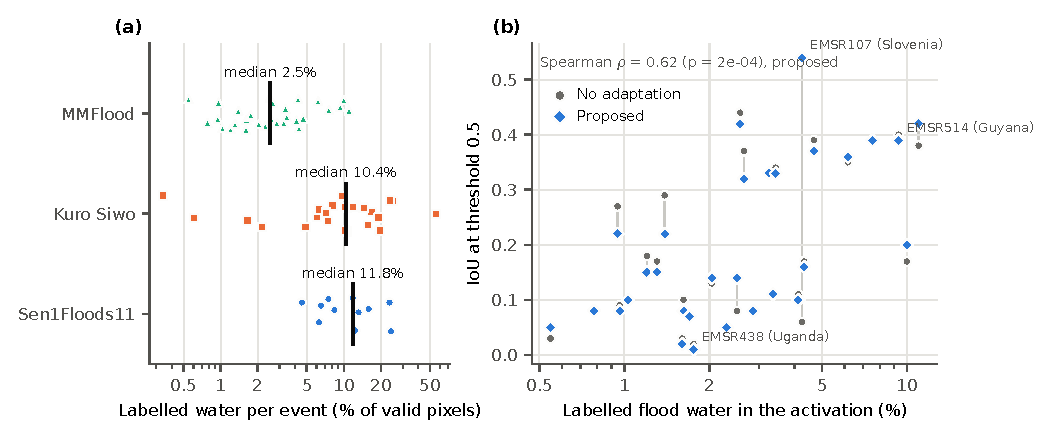
\includegraphics[width=\textwidth]{figures/fig_mmflood_water_audited.pdf}
\caption{(a) Water prevalence by evaluation unit (log scale, bars mark medians). Sen1Floods11 and Kuro Siwo use all-water support. MMFlood uses floodwater labels. (b) MMFlood: IoU at threshold 0.5 per activation against its water share, without adaptation and with the proposed method (mean over three models).}
\label{fig:mmwater}
\end{figure}

\section{External follow-up verification}

\subsection{GEOID-Flood ResNet-50 score readback}
The post-hoc crossover used the frozen v4 424-window selection from nine activations. Input verification recovered 1,416 selected radar, DEM, HAND and label raster hashes. CPU readback reconstructed the floodwater and dry label arrays from the archived rasters. It checked all 162 score digests and recomputed AP, source-threshold confusion counts and recall at matched false alarms. Table~\ref{tab:geoid_resnet_all} reports all six arms. Darkness-only and joint self-training share the positive teacher threshold, model, checkpoints, source normalisation and optimisation. The terrain gates are the only cue difference in this comparison. Joint physics improved AP over darkness alone on six of nine activations, with a mean gain of 0.20 points and a 95\% paired activation bootstrap interval of $-0.16$ to 0.72 points.

\begin{table}[pos=t]
\centering
\caption{Verified post-hoc GEOID-Flood ResNet-50 comparison. Metrics are percentages, averaged across the three checkpoints within each of nine activations, then across activations. IoU, miss and FPR use the fixed source threshold 0.430. The last two columns interpolate each activation--checkpoint ROC curve using reference labels.}
\label{tab:geoid_resnet_all}
\begin{tabular}{@{}lrrrrrr@{}}
\toprule
Method & AP & IoU & Miss & FPR & Recall at 2\% FPR & Recall at 5\% FPR \\
\midrule
Source only & 64.58 & 40.77 & 26.72 & 4.95 & 65.71 & 77.28 \\
AdaBN & 65.56 & 42.87 & 27.73 & 4.28 & 65.49 & 76.56 \\
Same-rule post-processing & 65.95 & 43.08 & 27.26 & 4.30 & 66.52 & 77.24 \\
Ordinary self-training & 66.39 & 45.72 & 30.35 & 3.75 & 65.71 & 77.39 \\
Darkness-only self-training & 67.38 & 44.67 & 26.87 & 4.23 & 66.95 & 78.31 \\
Joint physics-guided self-training & 67.58 & 45.12 & 27.26 & 4.12 & 67.10 & 78.69 \\
\bottomrule

\end{tabular}
\end{table}

\subsection{ImpactMesh controls and archived scores}
The relaxed ordinary comparison used the three original SSL4EO-S12 source checkpoints and the original 516 chips. It decreased the positive pseudo-label cutoff to 0.70 and kept the dry cutoff at 0.10. All 39 score arrays passed hash and reference-mask checks. The primary follow-up comparison used the earlier Kaggle ordinary and joint arms on the same Tesla T4 and software stack. The original frozen comparison gave the same direction of AP and matched-recall gains.

For the acquisition-time sensitivity, we retained chips acquired within three days of activation issuance and recomputed AP from the stored predictions. Gains were 16.30 points on average and 9.76 points at the median, with improvement on 11 of 12 scorable activations. Excluding EMSR848 gave 13.68 mean points, 7.63 median points and improvement on 10 of 11. A separate full-activation filter based on the median chip lag retained nine activations, excluded EMSR848 and gave a 15.51-point mean gain with eight improvements. Adaptation used the original chips. The filters changed only the scoring subset.


\clearpage
\bibliographystyle{unsrtnat}
\bibliography{references,audit_refs,external_refs}
\end{document}
